\section{Computed Properties}\label{computed-properties}

\begin{itemize}
\item
  Assumono valori dinamici in base ad altre property del nostro oggetto
  Vue;
\item
  Possono essere utilizzate come normali proprietà del campo data;
\end{itemize}

Usare le computed properties conviene perché usa la \emph{cache}, e i
nuovi valori vengono calcolati solo se e quando le dipendenze dovessero
cambiare.

Utilizzare le computed piuttosto che i metodi, evita di generare i
valori di ritorno ad ogni accesso, così da rigenerarli solo se e quando
le dipendenze dovessero cambiare (\emph{caching}).

Vengono utilizzate per calcolare il valore di una proprietà in base ad
alcune altre condizioni.

\section{Watchers}\label{watchers}

Si può usare questa opzione per attivare una funzione ogni volta che una
proprietà cambia.

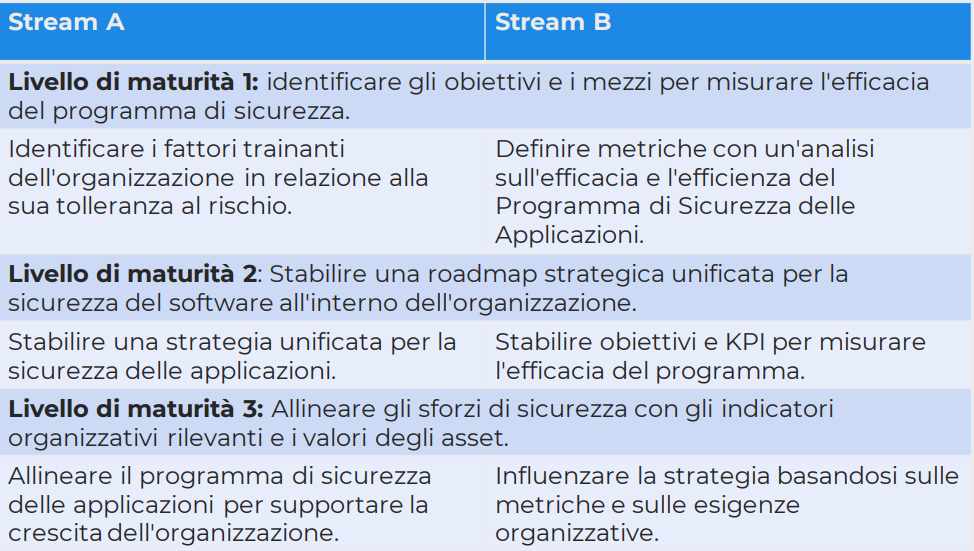
\includegraphics[width=6.26772in,height=2.52778in]{media/image13.png}

\section{Componenti}\label{componenti}

I componenti ci consentono di suddividere l\textquotesingle interfaccia
utente in parti indipendenti e riutilizzabili e di pensare a ogni parte
isolatamente, per farlo possiamo:

\begin{itemize}
\item
  utilizzando un custom tag: \emph{\textless hello-world
  /\textgreater{}}
\item
  utilizzando il tag component e l'attributo is:
  \emph{\textless component :is=''HelloWorld'' /\textgreater{}}
\end{itemize}

Possiamo registrarli:

\begin{itemize}
\item
  \textbf{Globalmente}: ma ciò impedisce di rimuovere i componenti
  inutilizzati e rende le relazioni di dipendenza meno esplicite.
\item
  \textbf{Localmente}: rende disponibile il componente solo
  all\textquotesingle interno del componente in cui è registrato
\end{itemize}

\section{Props}\label{props}

Rappresentano attributi custom che permettono di configurare un
componente dall\textquotesingle esterno, definite a priori, è possibile
definire il loro tipo o l'eventualità.

Passate ad un componente in maniera statica o dinamica.

Vue implementa il cosiddetto \textbf{one-way data flow}, le prop passate
ad un componente possono essere modificate dall'esterno, ma non dal
componente stesso, in quanto il flusso di dati è monodirezionale,
dall'alto al basso.

Risolvibile grazie agli eventi custom, è possibile per un componente
comunicare informazioni verso l\textquotesingle esterno, con
l\textquotesingle opzione emits un componente può definire a priori gli
eventi che è in grado di emettere e generare eventi.

Il cosiddetto \textbf{Prop Drilling} è quando dobbiamo passare una prop
da un componente A ad uno C e per farlo lo passiamo a B che è in mezzo.

Possiamo evitarlo con il \textbf{Provide - Inject}, dove A usa
l\textquotesingle opzione \emph{provide} per fornire dati a tutti i suoi
discendenti e C usa \emph{inject} per ottenere dati forniti tramite
provide da qualsiasi componente ascendente e utilizzarli come normali
properties.

\emph{\textbf{\ul{Nel progetto abbiamo preferito usare gli eventbus
perché i componenti non hanno una gerarchia diretta.}}}

\section{Slots}\label{slots}

Come le props ma per passare codice HTML fra componenti.

\section{Composition API}\label{composition-api}

Usate al posto delle \emph{Options API} (dividendo il codice nei blocchi
data, computed, methods, ecc.). I blocchi data, computed e methods sono
stati rimpiazzati dalla funzione setup(), che restituisce un oggetto
contenente tutte le variabili a cui il template deve avere accesso,
esiste ref che è grossomodo un equivalente di data.

Rispetto alle options API c'è maggior libertà
nell\textquotesingle organizzazione del codice, miglior supporto a
TypeScript e codice più compatto.

Aggiungendo l\textquotesingle attributo setup al tag
\textless script\textgreater{} il contenuto del tag diventi quello della
funzione setup().

Node.js

Una piattaforma software cross-platform che permette di creare il
proprio Web server.

Web application con connessioni real-time, two-way, dove non solo il
client, ma anche il server può iniziare una connessione, permettendo di
trasferire dati liberamente.

Usa un modello I/O non bloccante e ad eventi, che lo rende un framework
leggero ed efficiente, le richieste vengono tradotte in eventi (ognuno
dei quali è associato a un event handler) e inserite in una coda. C'è un
event loop single-threaded che controlla se ci sono nuovi eventi nella
coda.

Node.js è capace di gestire un elevato numero di connessioni simultanee.
Non congeniale per applicazioni CPU-intensive.

Node.js incorpora Node Package Manager (NPM), il più grande ecosistema
di librerie open source al mondo.

PHP

PHP è un linguaggio di scripting, interpretato, originariamente
concepito per la programmazione di pagine Web dinamiche lato server.

L'interprete PHP pre processa tutti i file con estensione PHP, che sono
sostanzialmente file contenenti HTML, all'interno dei quali è presente
del codice PHP, contenuto all'interno dei delimitatori
\emph{\textless?php \ldots{} ?\textgreater{}}. Ma è possibile anche
creare file con estensione \emph{.php} per poi includerli nel file
principale.

La sintassi PHP è di tipo C-like:

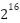
\includegraphics[width=4.03056in,height=2.30318in]{media/image3.png}

\section{Cookies}\label{cookies}

Sono un meccanismo di supporto alla gestione delle sessioni basato
sull'idea che sia il client a mantenere lo stato di precedenti
connessioni, e ad inviarlo al server di pertinenza ogni volta che
richiede un documento.

\emph{Il termine cookie indica un blocco di dati opaco lasciato dal
server in consegna ad un richiedente per poter ristabilire in seguito il
suo diritto alla risorsa richiesta .}

Alla prima richiesta di uno user-agent, il server fornisce la risposta
ed un header aggiuntivo, il cookie, con dati arbitrari e con la
specifica di usarlo per ogni successiva richiesta. Il server associa a
questi dati le informazioni sulla transazione. Ogni volta che lo
user-agent accederà a questo sito, rifornirà i dati opachi del cookie
che permettono al server di ri-identificare il richiedente, e creare
così un profilo specifico.

\subsection{Tipi}\label{tipi}

\begin{itemize}
\item
  \textbf{Tecnici}: usati dal gestore del sito per mettere in opera
  alcune funzioni o rendere più agile la navigazione;
\item
  \textbf{Analitici}: usati dal gestore del sito per raccogliere alcune
  informazioni in forma aggregata sugli utenti;
\item
  \textbf{Di profilazione}: sono usati dal gestore del sito per
  raccogliere dati personali sui visitatori {[}solo questi è necessario
  accettare{]}.
\end{itemize}

JavaScript Advanced

\section{API HTML5}\label{api-html5}

\subsection{WebStorage}\label{webstorage}

Le API WebStorage consentono di salvare e recuperare dati localmente al
browser, dati memorizzati in coppie chiave-valore.

Due oggetti principali:

\begin{itemize}
\item
  \textbf{localStorage}: i dati non hanno scadenza e non vengono
  cancellati alla chiusura del browser.
\item
  \textbf{sessionStorage}: a differenza di localStorage, i dati sono
  mantenuti solo per la sessione corrente e cancellati quando il browser
  viene chiuso.
\end{itemize}

A differenza dei cookies:

\begin{itemize}
\item
  Limite di memoria più ampio 10MB contro i 4MB dei Cookie.
\item
  Non ha una data di scadenza.
\item
  Non è possibile gestirli lato server.
\end{itemize}

\subsection{WebWorker}\label{webworker}

Permettono di eseguire codice Javascript in background.

\subsection{Drag and Drop}\label{drag-and-drop}

Le API Drag and Drop consentono di effettuare operazioni di drag and
drop all'interno della pagina.

\subsection{Geolocation}\label{geolocation}

L'API Geolocation consente di ottenere la posizione geografica
dell'utente.

\subsection{IndexedDB}\label{indexeddb}

Le API IndexedDB consentono di creare e manipolare un database
all'interno del browser, consentono di memorizzare quantità di dati
strutturati più grande rispetto alle API WebStorage.

\section{API JavaScript}\label{api-javascript}

\subsection{WebSocket}\label{websocket}

Le WebSocket consentono di instaurare un canale di comunicazione
full-duplex attraverso una singola connessione TCP.

\subsection{WebForms}\label{webforms}

Sono API per la validazione dei campi di input.

\subsection{WebHistory}\label{webhistory}

Web History fornisce un accesso facilitato all'oggetto windows.history,
che contiene gli URL visitati dall'utente.

\section{ECMAScript}\label{ecmascript}

Specifica tecnica di un linguaggio di scripting, standardizzata e
mantenuta da ECMA International nell\textquotesingle ECMA262 ed ISO/IEC
16262, la sua implementazione più conosciuta è Javascript.

Le versioni vanno da \textbf{ES2} a \textbf{ES6}.

L'ultima versione aggiunge \emph{Promise} che consente di gestire
l\textquotesingle eventuale completamento, o fallimento, di
un\textquotesingle operazione asincrona.

In una promessa, il valore non è necessariamente noto al momento della
creazione e la promessa consente di associare handler sia in caso di
successo che di errore di un'operazione asincrona; invece di restituire
il valore in modo sincrono, l'idea è quella di restituire la promessa di
fornire il valore in un momento futuro.

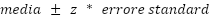
\includegraphics[width=6.26772in,height=2.27778in]{media/image1.png}

Un'altra aggiunta sono le \emph{async/await}, uno zucchero sintattico
che semplifica l'utilizzo delle funzioni asincrone e, di conseguenza,
anche delle Promise.

Mobile

Alcune definizioni:

\emph{Consiste in tecniche/tecnologie che permettono a utenti in
movimento di utilizzare device portatili, di eseguire applicazioni e di
connettersi ad applicazioni remote.}

\emph{È una tecnologia che consente la trasmissione di dati, voce e
video tramite un computer o qualsiasi altro dispositivo abilitato
wireless senza dover essere collegato ad un collegamento fisico fisso.}

\emph{È un termine generico che si riferisce a una varietà di
dispositivi che permettono alle persone di accedere a dati e
informazioni ovunque si trovino.}

Nel mobile bisogna rispettare alcune caratteristiche, come:

\textbf{Portabilità}: ridurre la dimensione dei dispositivi in modo da
creare computer che potessero essere portati in giro con relativa
facilità.

\textbf{Miniaturizzazione}: creare componenti hardware nuovi e molto
piccoli che permettano l'utilizzo del dispositivo personale durante uno
spostamento.

\textbf{Connettività}: sviluppare dispositivi e applicazioni che
permettessero all'utente di essere online e di comunicare wireless
durante gli spostamenti.

Bluetooth Low Energy (BLE) è una tecnologia di rete personale senza fili
che mira a nuove applicazioni nel settore sanitario, fitness, beacon
(trasmettitori hardware che trasmettono il loro identificatore ai
dispositivi elettronici portatili vicini.), sicurezza e intrattenimento
domestico.

\textbf{Convergenza :} integrare tutti i dispositivi esistenti in un
unico dispositivo ibrido in grado di fare tutto.

\textbf{Divergenza}: ogni dispositivo è pensato per svolgere una
specifica funzione.

Altri attori possono essere:

\textbf{Mobile communication}: infrastruttura creata per garantire una
comunicazione continua e affidabile per lo scambio di dati e voce
utilizzando reti wireless.

\textbf{Hardware mobile}: dispositivo di elaborazione portatile con la
capacità di recuperare ed elaborare i dati.

\textbf{Software mobile}: è il programma software che è stato sviluppato
specificamente per essere eseguito su hardware mobile.

Alcuni problemi da affrontare nel mobile sono:

\begin{itemize}
\item
  I dispositivi mobile sono «resource-constrained».
\item
  La connettività mobile è altamente variabile in termini di prestazioni
  e affidabilità.
\item
  I dispositivi mobili sono intrinsecamente meno sicuri, inoltre nuove
  problematiche dovute alla privacy.
\end{itemize}

\section{Sviluppo mobile}\label{sviluppo-mobile}

Conviene scegliere nativo o ibrido? Dipende da:

\begin{itemize}
\item
  Che tipo di app deve essere sviluppata;
\item
  Esigenze degli utenti.
\end{itemize}

\subsection{Native}\label{native}

Applicazioni sviluppate appositamente per un sistema operativo,
utilizzando il suo linguaggio di sviluppo.

Vantaggi:

\begin{itemize}
\item
  High performance
\item
  Sicurezza
\item
  Personalizzazione (UX)
\item
  Forte compatibilità con altre app
\item
  Assoluta compatibilità con API fornite dal OS
\end{itemize}

Svantaggi:

\begin{itemize}
\item
  Costo
\item
  Tempistiche
\end{itemize}

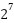
\includegraphics[width=3.88021in,height=2.45575in]{media/image11.png}

\subsection{(Responsive) Web app}\label{responsive-web-app}

È possibile accedere alle web app tramite il browser del dispositivo
mobile, non è necessario scaricare e installare l\textquotesingle app su
un dispositivo mobile per usarle, sviluppata come pagine Web e può
essere utilizzata sulla maggior parte dei dispositivi in grado di
navigare sul web.

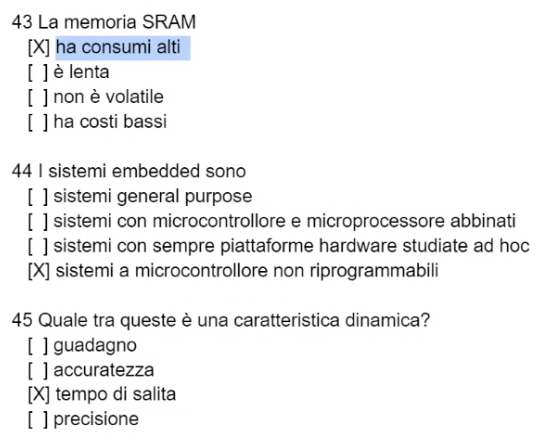
\includegraphics[width=4.05712in,height=2.10409in]{media/image8.png}

Queste applicazioni Web sono utilizzabili in qualsiasi dimensione del
riquadro di visualizzazione del browser (usabilità).

\subsection{Progressive Web App}\label{progressive-web-app}

Un\textquotesingle applicazione Web progressiva (PWA) è distribuita
attraverso il Web e creata utilizzando tecnologie web.

\emph{Sono app web che simulano il comportamento delle app mobili
native}

Utilizzano funzionalità della piattaforma Web in combinazione con il
miglioramento progressivo per offrire agli utenti
un\textquotesingle esperienza pari a quella delle app native.

Per \textbf{progressively enhanced} si intende una strategia nel web
design che pone l\textquotesingle accento sul contenuto, consentendo a
tutti di accedere al contenuto e alle funzionalità di base, mentre gli
utenti con funzionalità del browser aggiuntive o un accesso a Internet
più rapido ricevono la versione avanzata.

Questa strategia prevede la separazione del contenuto dalla
presentazione.

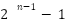
\includegraphics[width=4.43569in,height=2.50521in]{media/image10.png}

\subsection{Ibrido}\label{ibrido}

Le app mobili ibride sono applicazioni installate su un dispositivo,
proprio come qualsiasi altra app, ciò che le differenzia è il fatto che
combinano elementi da app native con elementi da app Web.

Distribuite in un contenitore nativo che usa un oggetto WebView mobile.
Quando si utilizza l\textquotesingle app, questo oggetto visualizza i
contenuti web grazie all\textquotesingle utilizzo di tecnologie web.

\section{Come sviluppare app}\label{come-sviluppare-app}

Ecco alcune tecnologie:

\begin{itemize}
\item
  \textbf{Flutter}: creato da Google, utilizzato per sviluppare
  applicazioni multipiattaforma, usa Dart come linguaggio;
\item
  \textbf{React Native}: create da Facebook, utilizzato per sviluppare
  applicazioni Android e iOS, usa JavaScript e tecnologie web;
\item
  \textbf{Ionic Framework}: è un toolkit
  dell\textquotesingle interfaccia utente open source per la creazione
  di app mobili e desktop performanti e di alta qualità utilizzando
  tecnologie Web, consente di creare app per tutti i principali app
  store da un\textquotesingle unica base di codice, nativo e ottimizzato
  per il web;
\item
  \textbf{Cordova}: framework di sviluppo mobile open source di Apache
  che utilizza le tecnologie web;
\item
  \textbf{Capacitor}: progetto open source che esegue app Web moderne in
  modo nativo su iOS, Android e Web.
\end{itemize}

Data Visualization

Quando si usano i dati per mostrare o spiegare qualcosa in maniera
visiva, esempio:

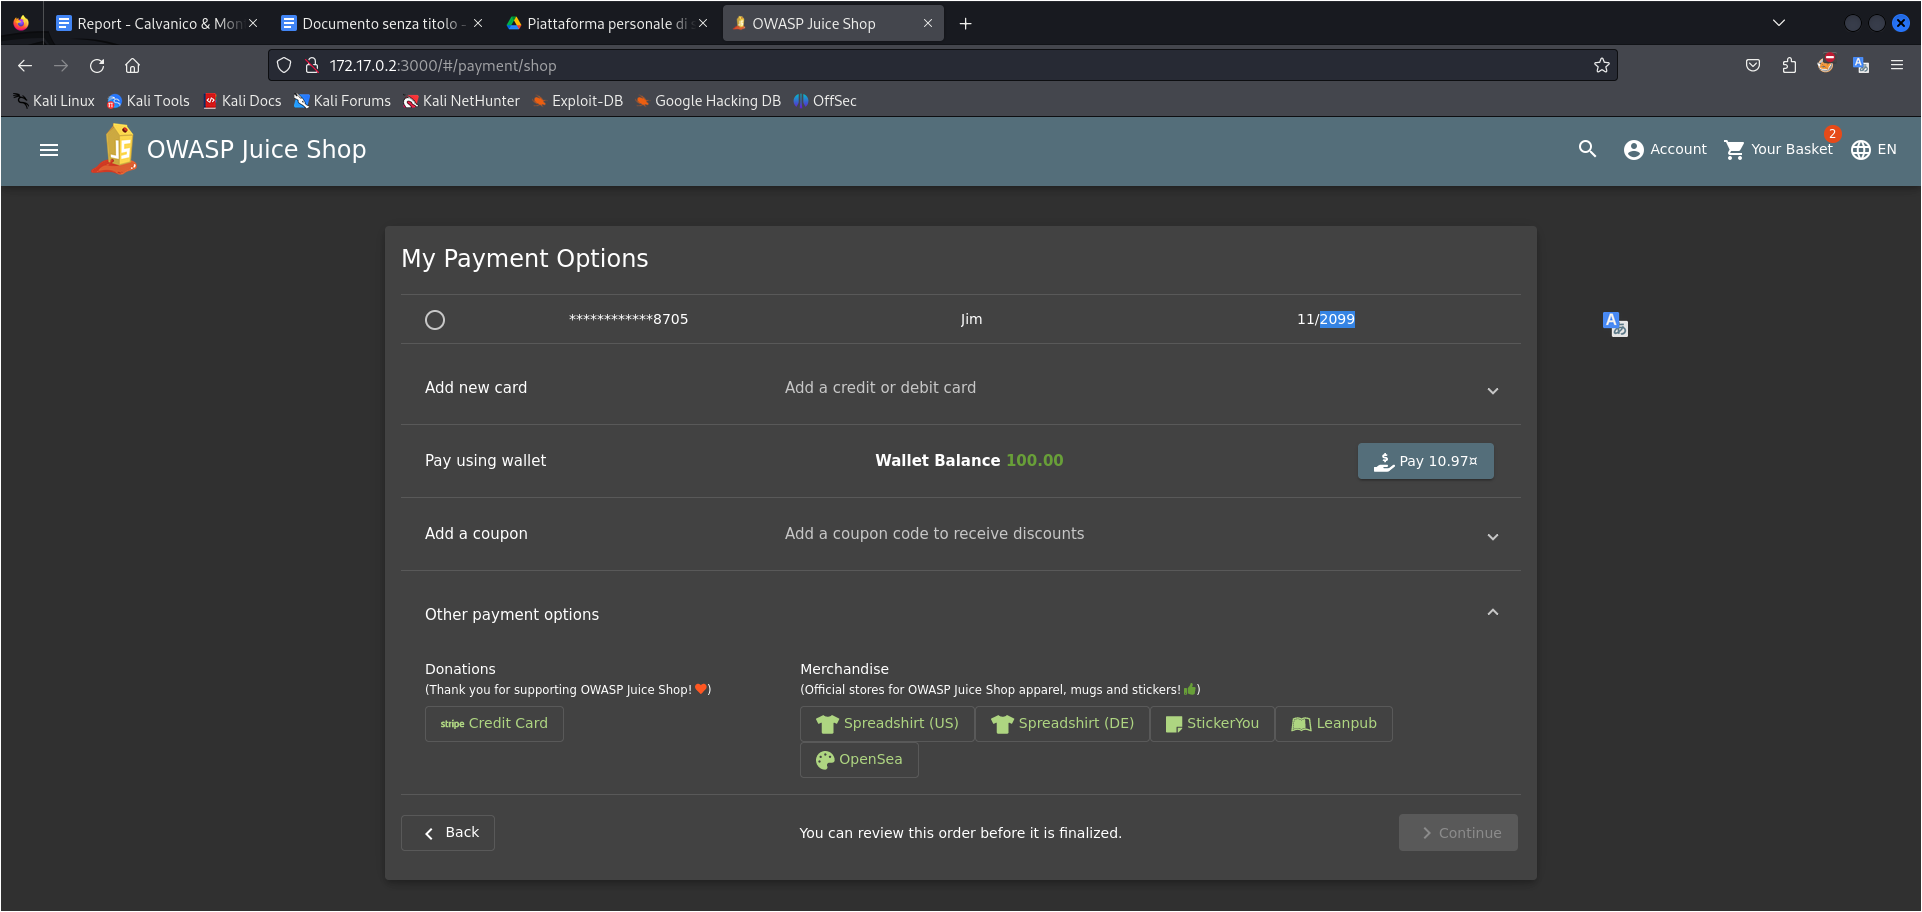
\includegraphics[width=4.11893in,height=2.90104in]{media/image12.png}

Si usa perchè: l\textquotesingle idea della visualizzazione ci aiuta a
vedere ciò che non abbiamo notato prima. Particolarmente vero quando si
cerca di identificare le relazioni e di trovare un significato in enormi
quantità di dati raccolti (cioè i Big Data).

\textbf{Visualization}: qualsiasi tipo di rappresentazione visiva di
informazioni progettata per consentire la comunicazione,
l\textquotesingle analisi, la scoperta, l\textquotesingle esplorazione,
la trasmissione di un messaggio, ecc.

\textbf{Information Visualization}: studio delle rappresentazioni visive
di dati astratti ( sia dati numerici che non numerici) per rafforzare la
cognizione umana.

\textbf{Infografica}: rappresentazione visiva di informazioni in più
sezioni con lo scopo di comunicare uno o più messaggi specifici.
\emph{Con lo \textbf{scopo} di rendere i dati facilmente comprensibili a
colpo d\textquotesingle occhio o con una breve attenzione}.

\textbf{Data visualization}: rappresentazione grafica di informazioni e
dati.

\section{\texorpdfstring{\textbf{Qualità delle buone
visualizzazioni}:}{Qualità delle buone visualizzazioni:}}\label{qualituxe0-delle-buone-visualizzazioni}

\begin{enumerate}
\def\labelenumi{\arabic{enumi}.}
\item
  \emph{Truthful\textbf{: }}essere onesti facendo le giuste scelte di
  design.
\item
  \emph{Functional}: scegliere le forme grafiche in base ai compiti che
  si desidera permettere di fare.
\item
  \emph{Beautiful}: gli oggetti devono essere o vissuti come belli dal
  maggior numero possibile di persone.
\item
  \emph{Insightful}: le buone visualizzazioni aprono la strada a
  scoperte preziose che sarebbero inaccessibili se le informazioni
  fossero presentate in un modo diverso.
\item
  \emph{Enlightening}: qualità composta dalle quattro precedenti.
\end{enumerate}

\section{Processo di visualizzazione dei
dati}\label{processo-di-visualizzazione-dei-dati}

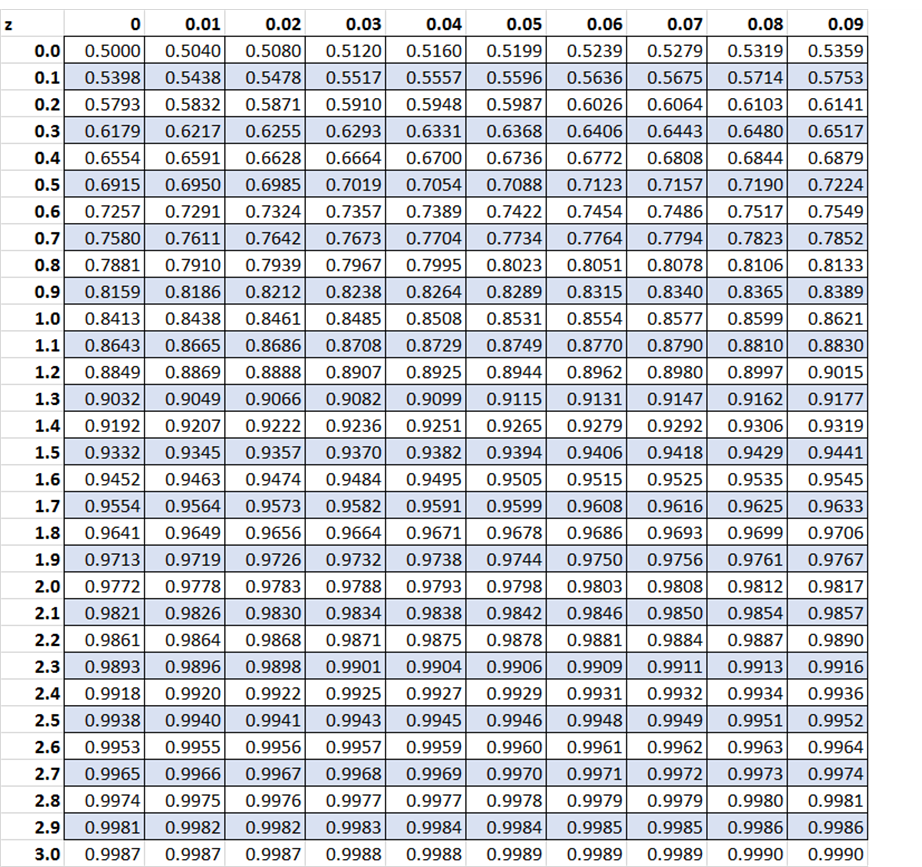
\includegraphics[width=6.26772in,height=0.98611in]{media/image9.png}

I dati possono essere:

\begin{itemize}
\item
  \textbf{Categorici}: descrivono categorie o gruppi
\item
  \textbf{Numerici}: rappresentano numeri (quantità, range ecc..)
\end{itemize}

Per la visualizzazione esistono diversi grafici:

\begin{itemize}
\item
  \textbf{Bar chart}: per comparare più valori, se modifichiamo troppo
  la scala manipoliamo le informazioni.
\end{itemize}

\begin{quote}
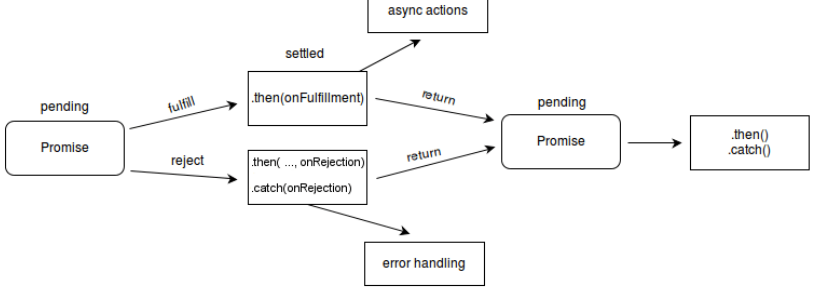
\includegraphics[width=4.4545in,height=1.94607in]{media/image7.png}
\end{quote}

\begin{itemize}
\item
  \textbf{Istogramma}: rappresentazione grafica di una distribuzione di
  una variabile numerica. \emph{Asse X: \textbf{intervalli}} invece
  \emph{Asse Y: \textbf{frequenza}}.
\end{itemize}

\begin{quote}
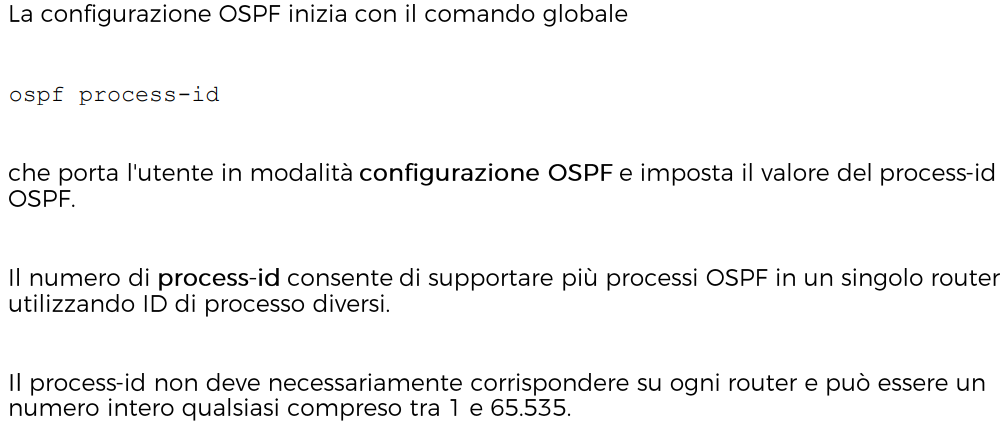
\includegraphics[width=1.86352in,height=1.42188in]{media/image4.png}
\end{quote}

\begin{itemize}
\item
  \textbf{Grafico a torta}: usato per rappresentazioni di variabili
  quantitative misurate su classi di categorie, circolare per evitare un
  ordine, ha il difetto che \emph{la dimensione delle slice non è un
  facilmente leggibile}. \textbf{NON} è la scelta migliore.
\item
  \textbf{Treemap}: visualizza i dati gerarchici come un insieme di
  rettangoli annidati.
\end{itemize}

\begin{quote}
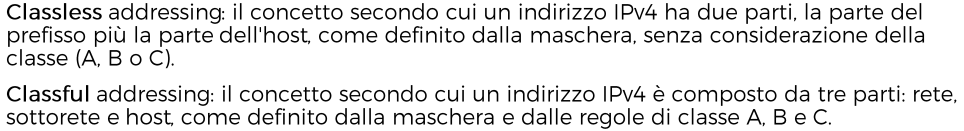
\includegraphics[width=2.69948in,height=1.0844in]{media/image6.png}
\end{quote}

\begin{itemize}
\item
  \textbf{Area chart}: descrivono i cambiamenti delle variabili nel
  tempo
\end{itemize}

\begin{quote}
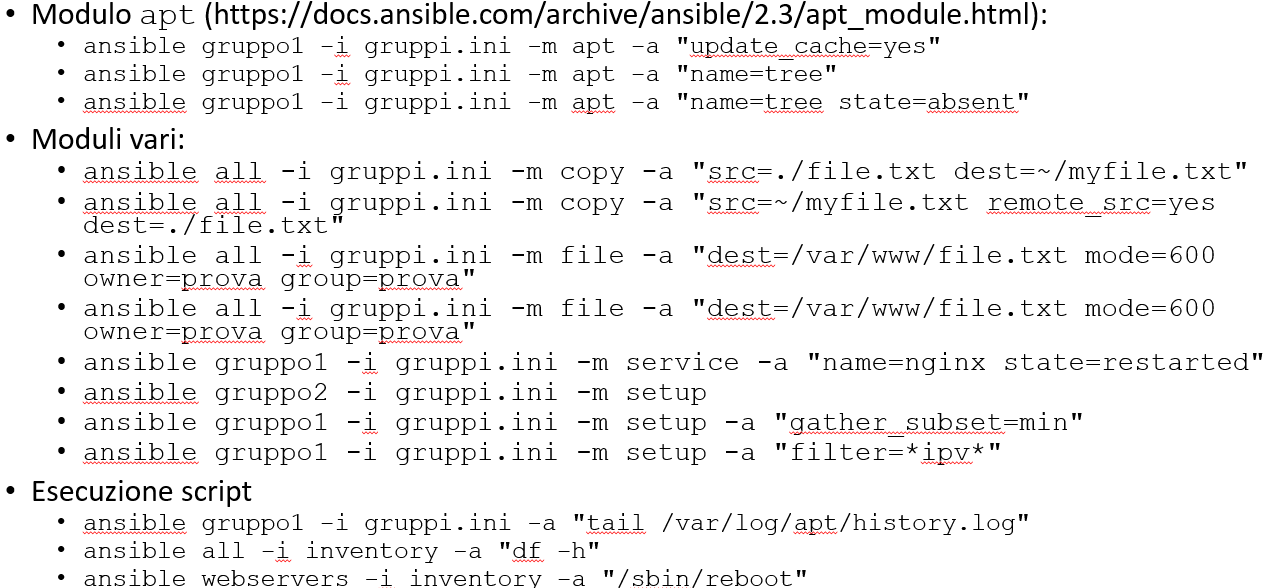
\includegraphics[width=2.34916in,height=1.7132in]{media/image2.png}
\end{quote}

\begin{itemize}
\item
  \textbf{Stacked area chart}:
\end{itemize}

\begin{quote}
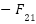
\includegraphics[width=2.41845in,height=1.66077in]{media/image14.png}
\end{quote}

\begin{itemize}
\item
  \textbf{Line chart}: utilizzati per rappresentare i dati delle serie
  temporali. È adatto a mostrare dati che cambiano in modo continuo.
\end{itemize}

\begin{quote}
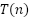
\includegraphics[width=2.5535in,height=1.3334in]{media/image5.png}
\end{quote}

\begin{itemize}
\item
  \textbf{Scatter plot}: due variabili di un dataset sono riportate su
  uno spazio cartesiano, dati visualizzati tramite una collezione di
  punti.
\item
  \textbf{Bubble chart}: tipo di grafico in cui ogni entità
  rappresentata è definita in termini di tre parametri numerici
  distinti.
\item
  \textbf{Choropleth map}: usano i colori per rappresentare quantità e
  qualità di una certa area geografica i cui confini sono prestabiliti.
\item
  \textbf{Dot maps}: usano una stessa forma per rappresentare ogni
  singola unità di dati. Il risultato visivo è che le zone con maggiore
  densità risultano ricoperte da una quantità maggiore di punti.
\end{itemize}

\section{D3.js}\label{d3.js}

D3.js (Data-Driven Documents) è una libreria Javascript per produrre
visualizzazioni di dati dinamiche e interattive nei browser,
estremamente veloce e supporta comportamenti dinamici.

Gamification

\emph{``Gamification'' is the use of game design elements in non-game
contexts.}
